Several fully labeled and protected nanosphere samples were created during the '11--'12 year. The protocol used was adapted from Oliver Hoidn and Perry Ellis's report~\citep{hoidnellis}, using 2,000 antibodies per Au nanosphere and the curve-elbow value 10,000 PEG-SH molecules per Au nanosphere. Detailed documentation of the protocol can be found in \autoref{a:protocol}.

The progress of the protocol was monitored by a DLS radius measurement at five or six stages:

\begin{enumerate}
\item Immediately after the addition of the OPAb

\item 24 hours after the addition of the OPAb

\item Immediately after the addition of the PEG-SH

\item 24 hours after the addition of the PEG-SH

\item After dilution with equal parts PBS, to check for protection

\item (For most but not all samples) 48 hours after the addition of PEG-SH

\end{enumerate}

The results of these measurements are shown in \autoref{fullprotocol}. The data shows an immediate increase of 6--8 nm upon the addition of the OPAb, followed by slight ($<$0.1 nm) gains after 24 hours of incubation. AP124F is an IgG antibody and has dimensions of approximately $14.5\mathrm{\,nm}\times8.5\mathrm{\,nm}\times4.0\mathrm{\,nm}$~\citep{antibodylength} as shown in \autoref{iggstructure};
since the NHS replacement can occur on any lysine or N terminus (of which there are several), a 6--8 nm increase in radius is reasonable when all spatial orientations are taken into account.

\begin{figure}[htbp]
\centering
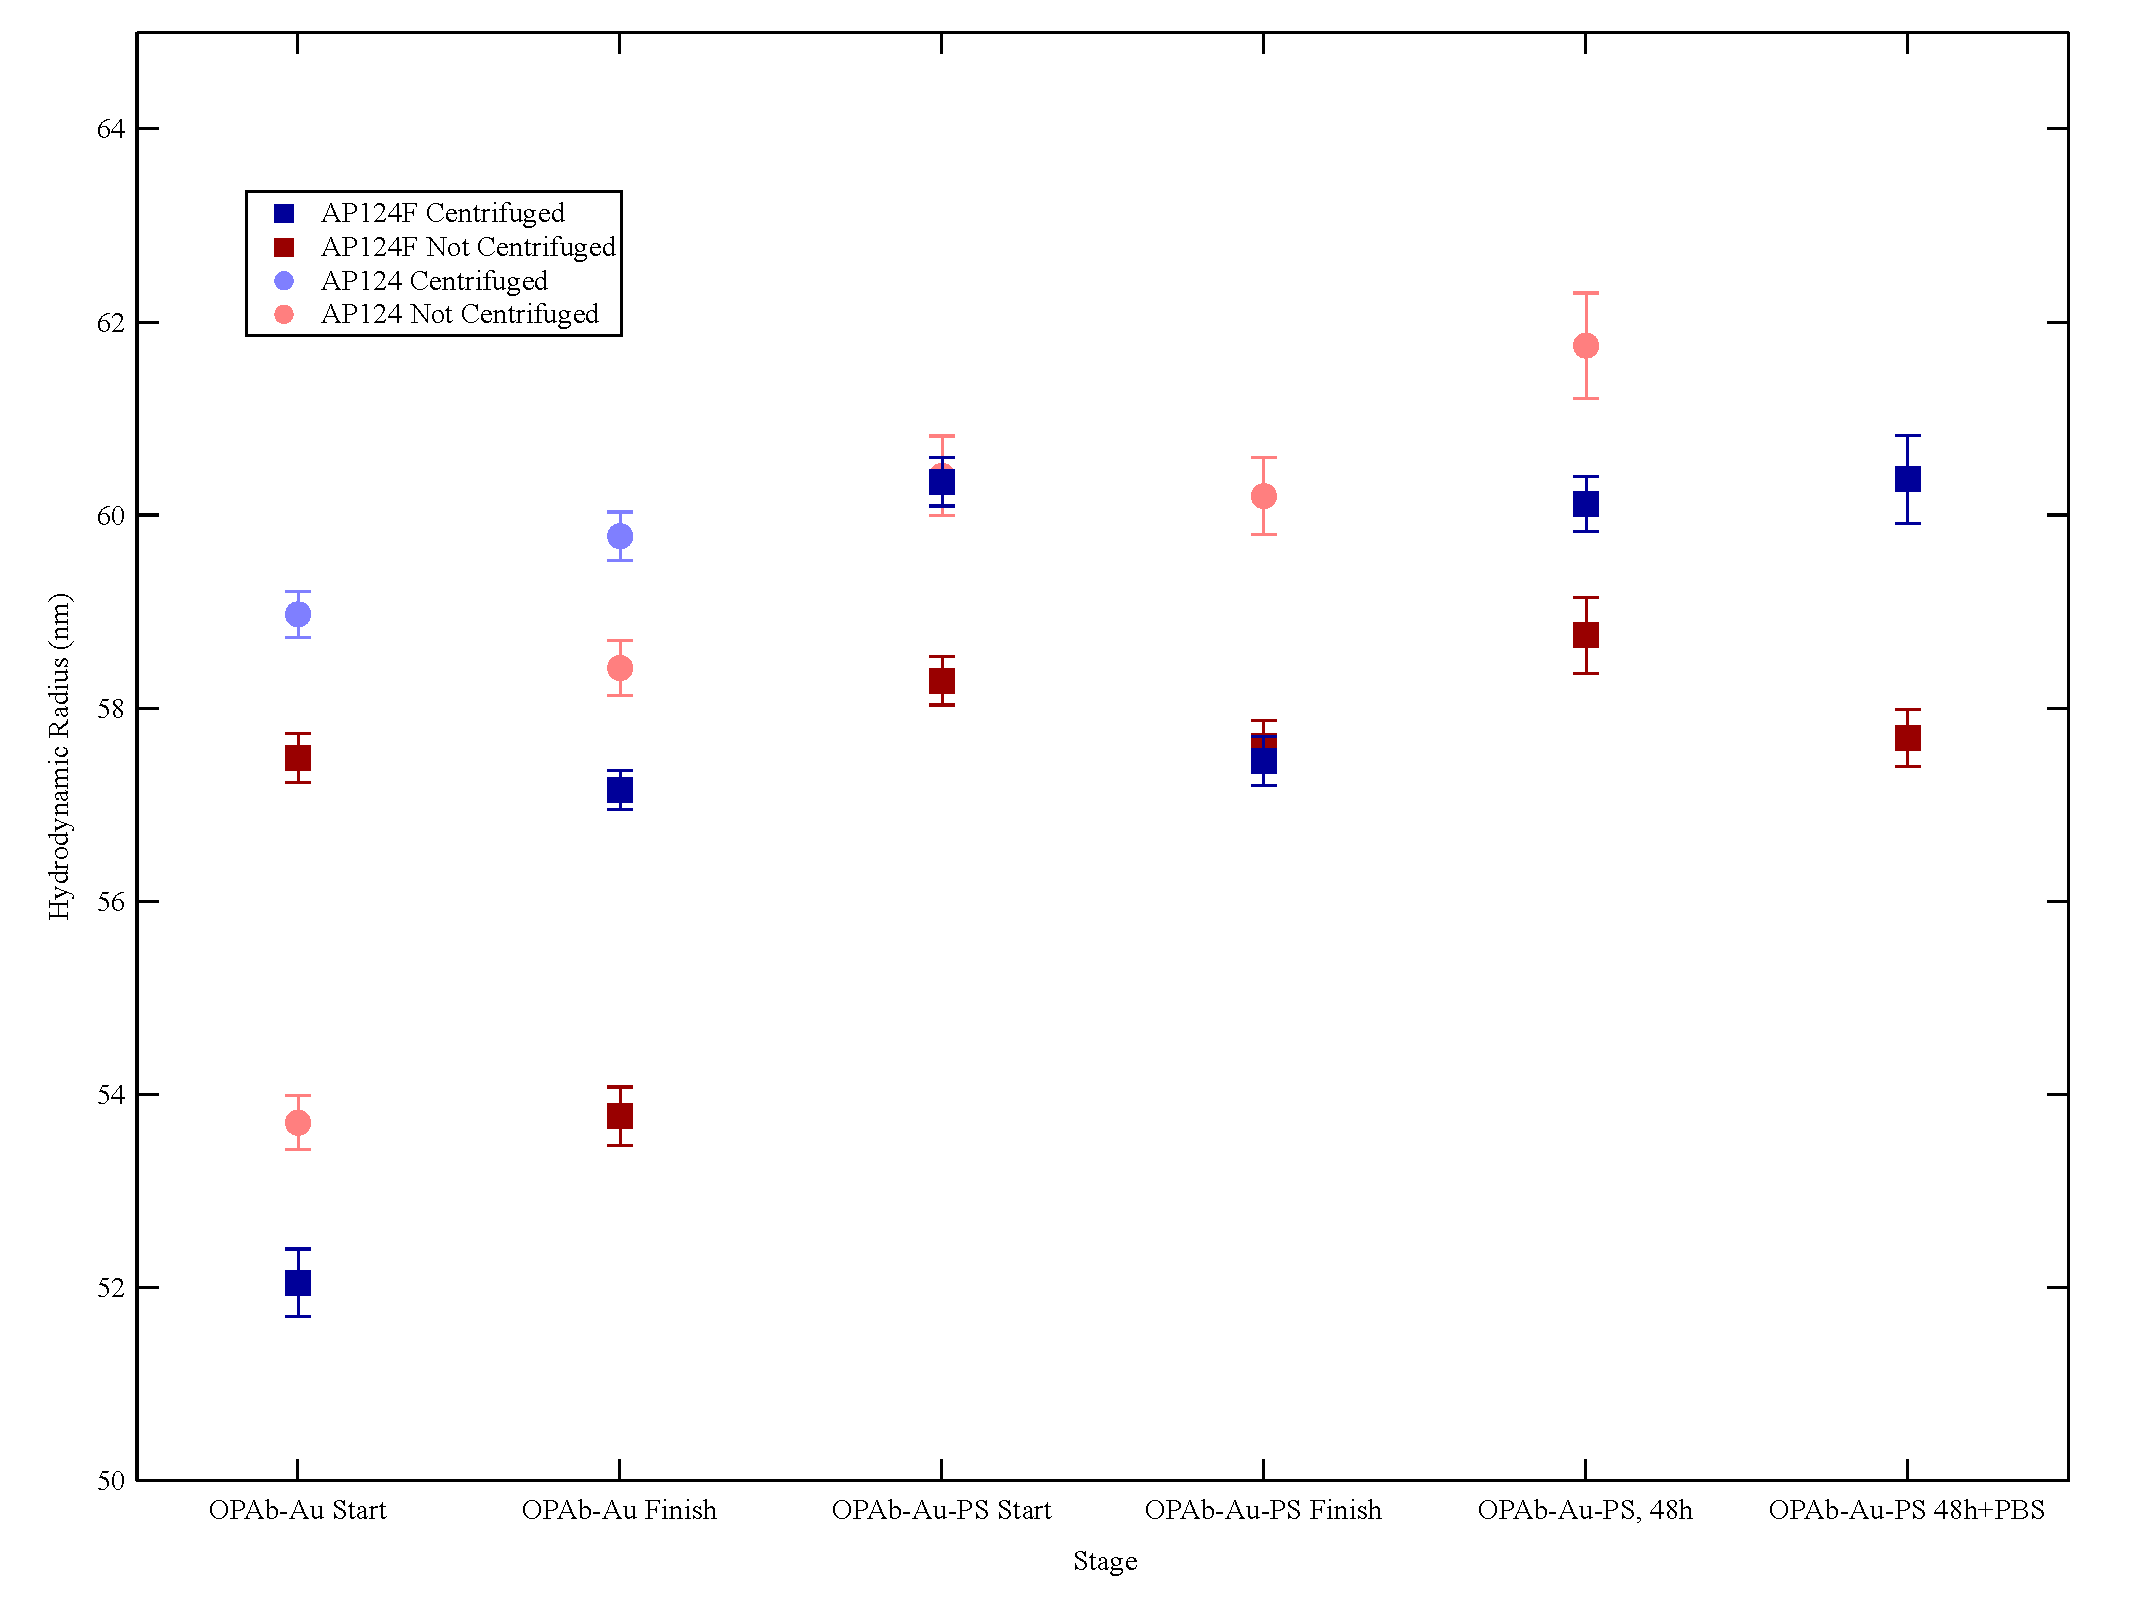
\includegraphics[keepaspectratio,width=\textwidth,height=0.75\textheight]{2011DecPEGylation.pdf}
\caption{Plot of hydrodynamic radii of multiple solutions at each step in the protocol. NOTE: PLACEHOLDER UNTIL I COLLATE ALL THE DATA.}
\label{fullprotocol}
\end{figure}



\begin{figure}[htbp]
\centering
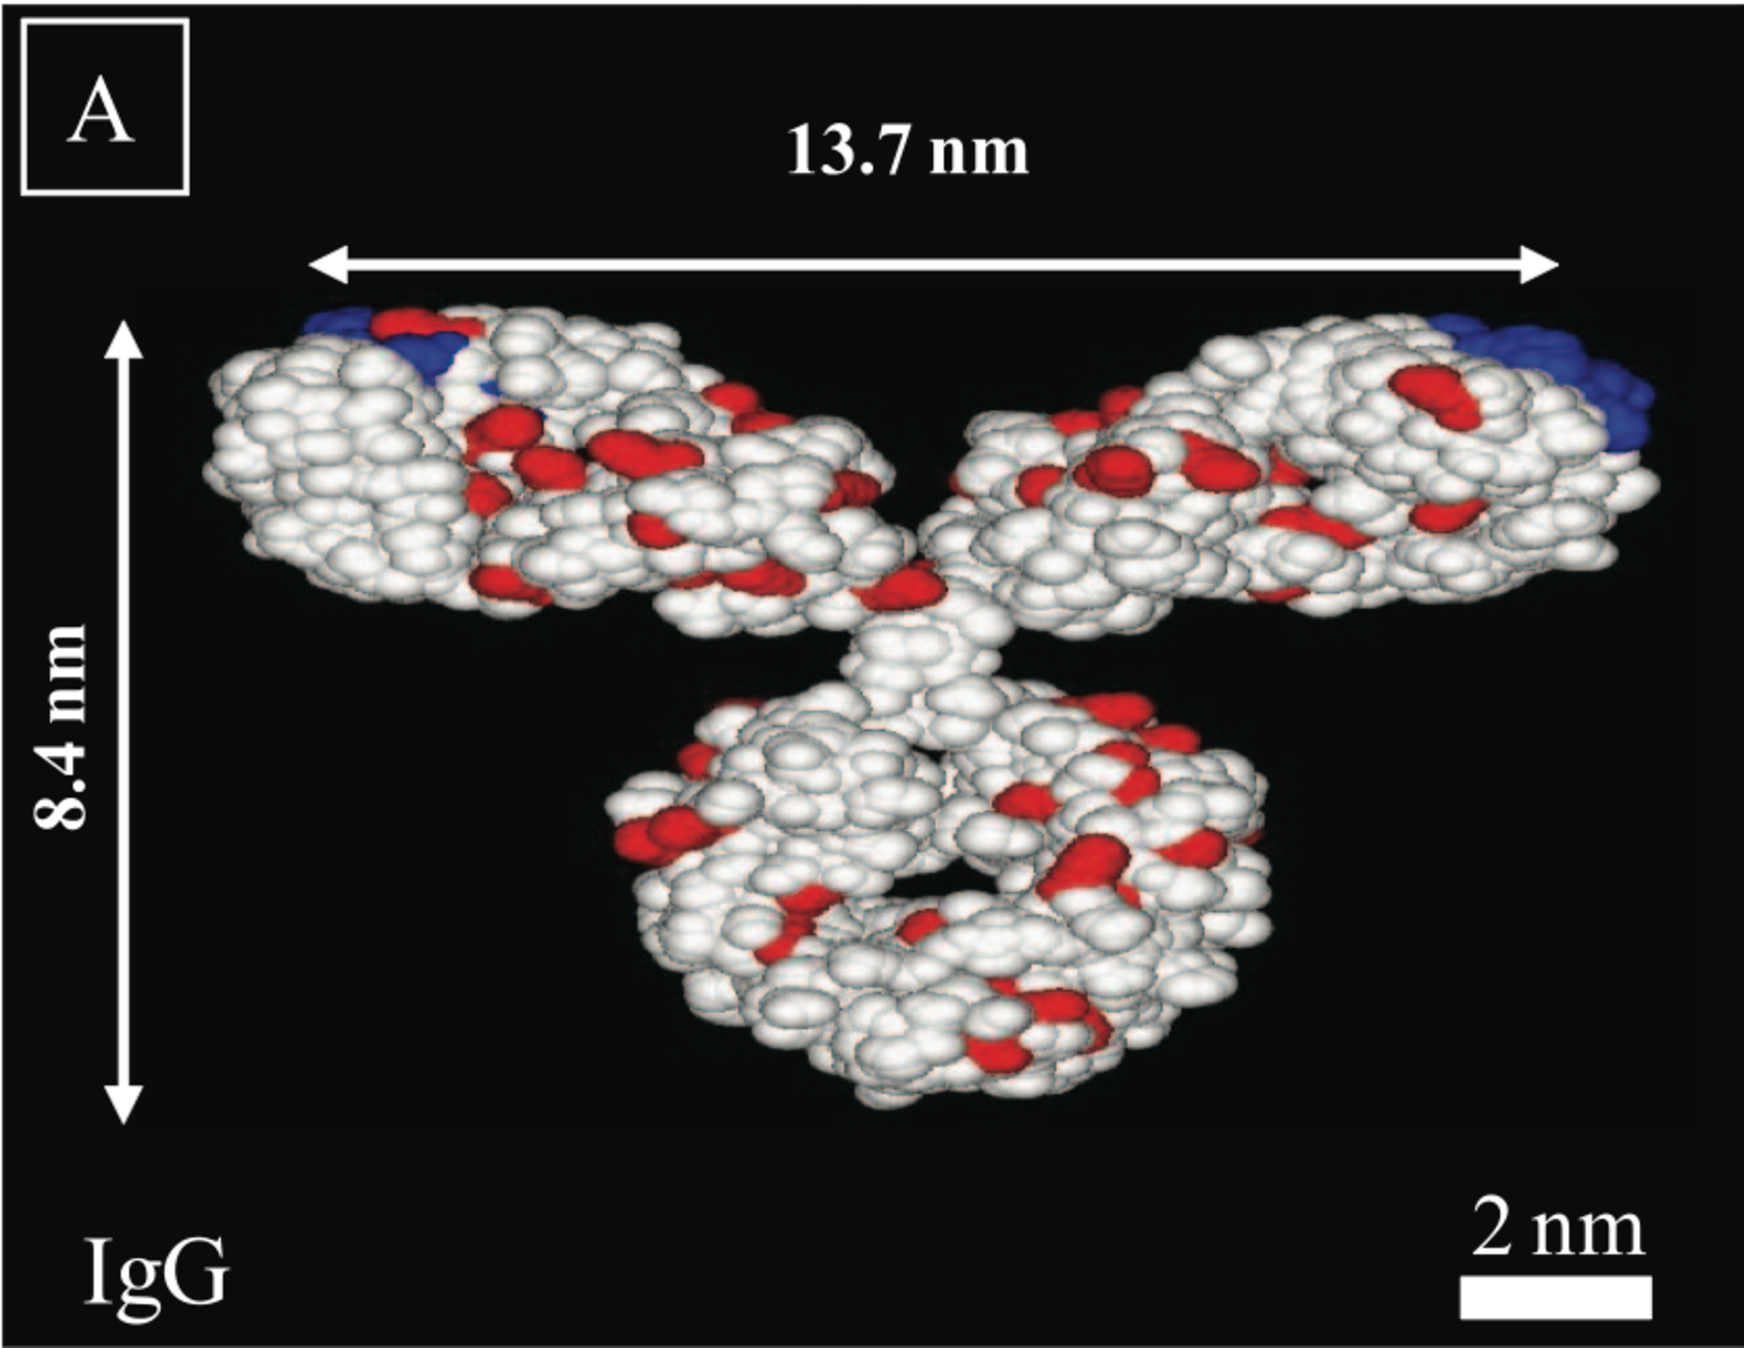
\includegraphics[keepaspectratio,width=3in,height=0.75\textheight]{iggstructure.pdf}
\caption{Structure dimensions of an IgG antibody. From ~\citep{antibodylength}.}
\label{iggstructure}
\end{figure}




Additional analysis can be performed by using the same number estimation as in \autoref{additionofpeg-shtonanospheres}. An OPAb conjugate should have a volume of
\[V=V_{\mathrm{PEG}}+V_{\mathrm{Ab}}=\frac{2.1\mathrm{kDa}}{1.11\frac{\mathrm g}{\mathrm cm^3}}+\frac{160\mathrm{kDa}}{1.35\frac{\mathrm g}{\mathrm cm^3}}=200\,\mathrm{nm}^3\]
Examining the hydrodynamic volume change after the addition of PEG-SH, this corresponds to
\[\frac{4}{3}\pi[(58\mathrm{\,nm})^3-(51.5\mathrm{\,nm})^3]/\frac{200\,\mathrm{nm}^3}{OPAb}=1230\mathrm{\ OPAb}\]
However, this may be an over-estimate, as the 1.35 $\mathrm{\frac{g}{cm^3}}$ density is for the crystalline state of protein~\citep{proteindensity}; the actual effective volume of the OPAb in solution may be larger. Further uncertainty is introduced by the complexity of the diffusion of an Au nanosphere with over 1000 OPAb molecules attached to it. Therefore, this calculation serves primarily as an order-of-magnitude check; in that sense, 1230 OPAb\slash Au compares quite favorably to the 2000 OPAb\slash Au in solution.

We can again perform a calculation of effective width: \[A_{\mathrm{OPN}}=\frac{4\pi(51.5\mathrm{\,nm})^2/\mathrm{Au}}{1230\mathrm{\frac{OPAb}{Au}}}=27.1\,\mathrm{nm}^2\]
This is considerably larger than the effective width of the PEG-SH, indicating that the OPAb molecules on the nanosphere sterically (word choice?) hinder other OPAb molecules from forming thiol bonds with the nanosphere surface. Since the binding mechanism between the PEG chain and the gold surface is the same, this means that there is likely additional room for thiol bonds on the surface, which means that that the PEG-SH should fill in gaps on the surface of the sphere.

Performing the same volumetric analysis on the change in radius from OPAb-Au to OPAb-Au-PS, we see that the number of PS molecules bound to the OPAb-Au is approximately
\[\frac{4}{3}\pi[(59\mathrm{\,nm})^3-(58\mathrm{\,nm})^3]/\frac{7.5\,\mathrm{nm}^3}{PS}=5730\mathrm{\ PS}.\]
This number is the right order of magnitude, given that 10,000 PS\slash Au were added, and only the gaps on the surface are expected to be filled.

The addition of PEG-SH brings the total number of thiol bonded PEG chains on the Au nanosphere surface to approximately 7,000. Though that is not quite the number of PEG-SH molecules that demonstrated protection in Ch.\autoref{additionofpeg-shtonanospheres}, the combination of the 7,000 PEG chains and the antibodies clearly protected the spheres from agglomeration. This is evidenced by the lack of radius increase when the fully labeled and protected nanospheres are diluted with an equal volume of commercial phosphate-buffered saline (PBS) solution, as shown in \autoref{fullprotocol}. Since the radial growth of the spheres matched its predicted behavior fairly well, the decision was made to progress to useing the nanospheres to label a cell culture monolayer.
